
\section*{GitHub Overview}

link to GitHub repository: \url{https://github.com/DPS-DistributedIntelligence/DPS-Project}

For this project, the implementation was done in a structured way, what do we mean by this, is that every implementation of testing was done in a separate branch from the main branch. This to avoid conflicts and provide a working branch through every commit done in the main branch.

This having as a result a total of 15 branches (including main branch implementation), where either development was done or testing as lested in Table \ref{tab:git_branches};

%%% git_branches
%\begin{figure}[ht]
%    \centering
%    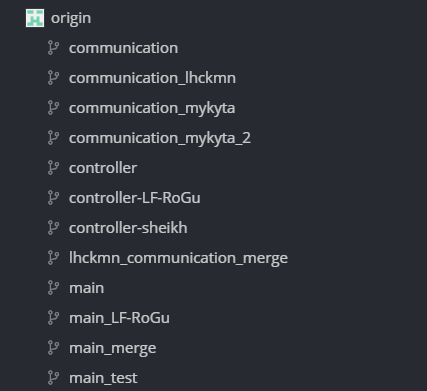
\includegraphics[width=0.5\textwidth]{images/git_branches.png}
%    \caption{git branches}
%    \label{img:git_branches}
%\end{figure}

\begin{table}
\centering
\caption{Git branches}
\begin{tabular}{|l|l|} 
\hline
Item        & Branche's Name  \\ 
\hline
1           & communication             \\ 
\hline
2           & communication\_lhckmn           \\ 
\hline
3           & communication\_mykyta            \\
\hline
4           & communication\_mykyta\_2             \\
\hline
5           & controller             \\
\hline
6           & controller-LF-RoGu             \\
\hline
7           & controller-sheikh             \\
\hline
8           & lhckmn\_communication\_merge             \\
\hline
9           & main             \\
\hline
10          & main\_LF-RoGu             \\
\hline
11          & main\_merge             \\
\hline
12          & main\_test             \\
\hline
\end{tabular}
\label{tab:git_branches}
\end{table}

\subsection{Line Of Code}

The number of lines and files are listed in Table \ref{tab:lines_of_code} and the language that we used is C++.

%\textbf{Lines Of Code}

%%% lines_of_code_summary
%\begin{figure}[ht]
%    \centering
%    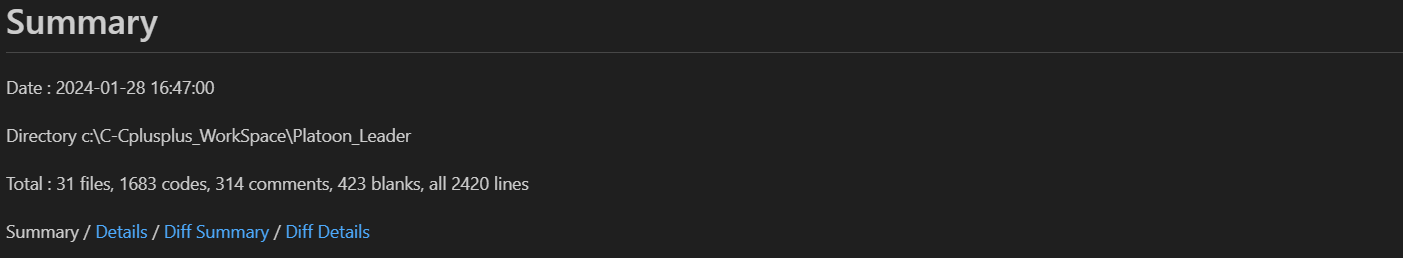
\includegraphics[width=0.5\textwidth]{images/lines_of_code_summary.png}
%    \caption{lines of code summary}
%    \label{img:lines_of_code_summary}
%\end{figure}


\begin{table}
\centering
\caption{lines of code summary}
\begin{tabular}{|l|l|} 
\hline
Item        & Amount  \\ 
\hline
Files       & 31             \\ 
\hline
Codes       & 1683           \\ 
\hline
Comments    & 314            \\
\hline
Blanks       & 423             \\
\hline
Lines       & 2420             \\
\hline
\end{tabular}
\label{tab:lines_of_code}
\end{table}




%%% lines_of_code_language
%\begin{figure}[ht]
%    \centering
%    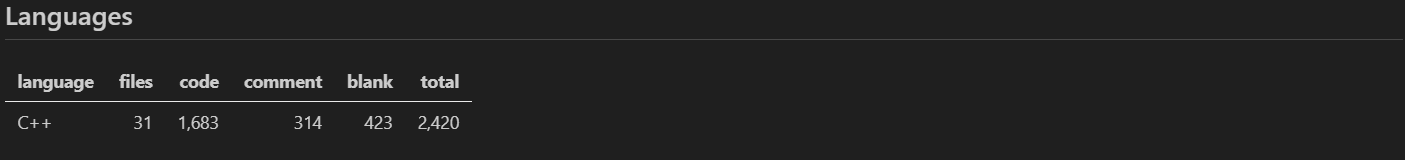
\includegraphics[width=0.5\textwidth]{images/lines_of_code_language.png}
%    \caption{lines of code language}
%    \label{img:lines_of_code_language}
%\end{figure}

\subsection{Code directory}
.
\dirtree{%
.1 \myfolder{DPS-project}.
.2 \myfolder{Code}.
.3 \myfolder{cmake-build-debug}.
.3 \myfolder{src}.
.2 \myfolder{Documentation}.
}.


The tree above arethe directory tree of our github reprository and the directory of \textit{src} folder are listed in Figure \ref{img:lines_of_code_directory}
%%% lines_of_code_directory
\begin{figure}[ht]
    \centering
    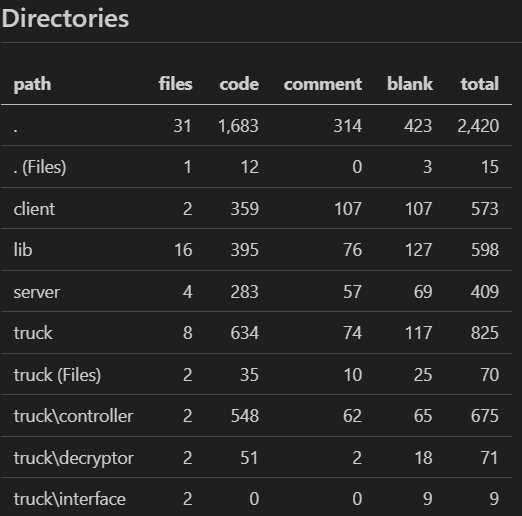
\includegraphics[width=0.5\textwidth]
   {images/lines_of_code_directory.png}
    \caption{lines of code directory}
    \label{img:lines_of_code_directory}
\end{figure}

In \textit{src} folder, you can find all the source code for the project. The option to simply add all the files in one "src" folder was made so we can simply update and add to the compilation rules the src folder.
\begin{enumerate}
    \item client - Source code for the client communication that the object "Truck" will have to connect to the server.
    \item lib - Source code for all enumerations, structures and headers that the project will need.
    \item server - Source code for the server to be able to run
    \item truck - Source code of all the items that the truck should have such as controller.
\end{enumerate}

\subsection{Amount of commits}
Since most of the implementation was done in branches, it will only be shown the most important branches of the implementation.
\begin{itemize}
    \item main, 86 commits
    \item communication, 14 commits
    \item communication-lhckmn, 28 commits
    \item communication-mykyta, 20 commits
    \item controller, 33 commits
    \item controller-LF-RoGu, 32 commits
    \item controller-sheikh, 33 commits
    \item threads, 33 commits
    \item truck-LF-RoGu, 18 commits
    \item main-merge, 77 commits
\end{itemize}
